\newpage

\section{Outline}

\subsection{Our Scope}

Our technology is the indelible GPT-3 series of Large Language Models (LLMs). Within this family of models, we apply a Value-Sensitive Design (VSD) analysis to:

\begin{itemize}
\item GPT-3 (the original 2020 paper)\footnote{\cite{gpt3}};
\item InstructGPT (a subsequent RLHF (Reinforcement Learning Human Feedback) iteration);\footnote{\cite{instructgpt}}
\item and finally ChatGPT (a sibling model of InstructGPT without an official corresponding paper).
\end{itemize}


\begin{figure}[h]
    \centering
    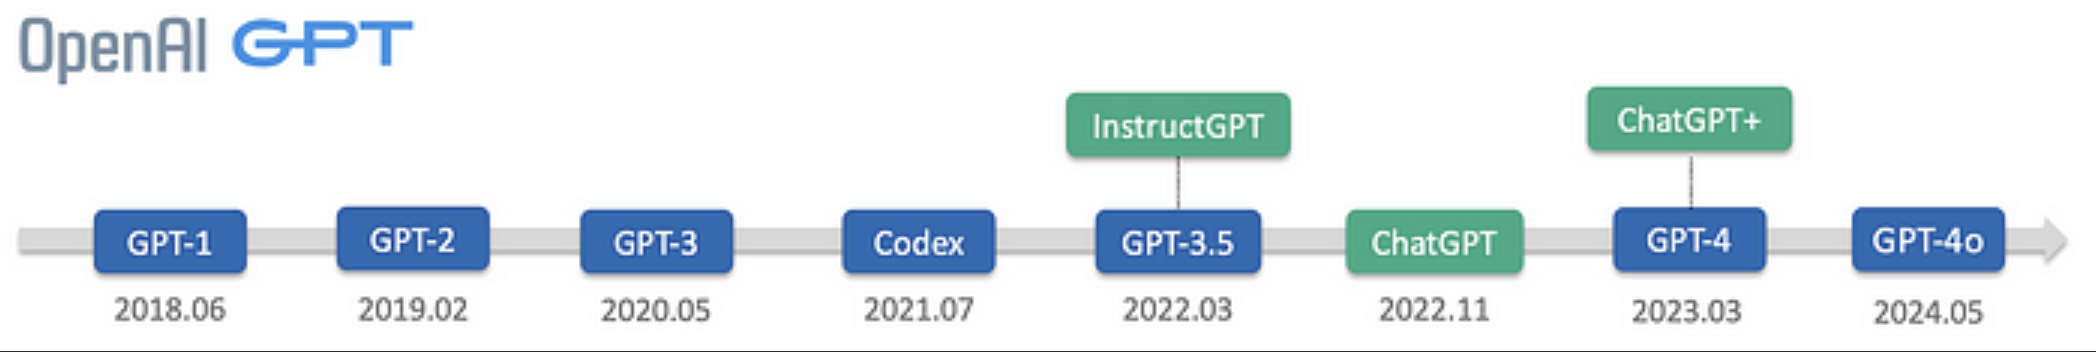
\includegraphics[width=0.8\textwidth]{aayushbajaj/Documents/uni/comp4920/group-project/report/img/gpt-timeline.png}
    \caption{OpenAI GPT iterations across time}
    \label{fig:image1}
\end{figure}

We consider the publicly released product at \href{https://openai.com/}{openai.com} on the 30th of November 2022 as the basis for our \hyperlink{section.2}{Stakeholder Analysis} and \hyperlink{section.4}{Comparative Analysis}.

\begin{figure}[h]
    \centering
    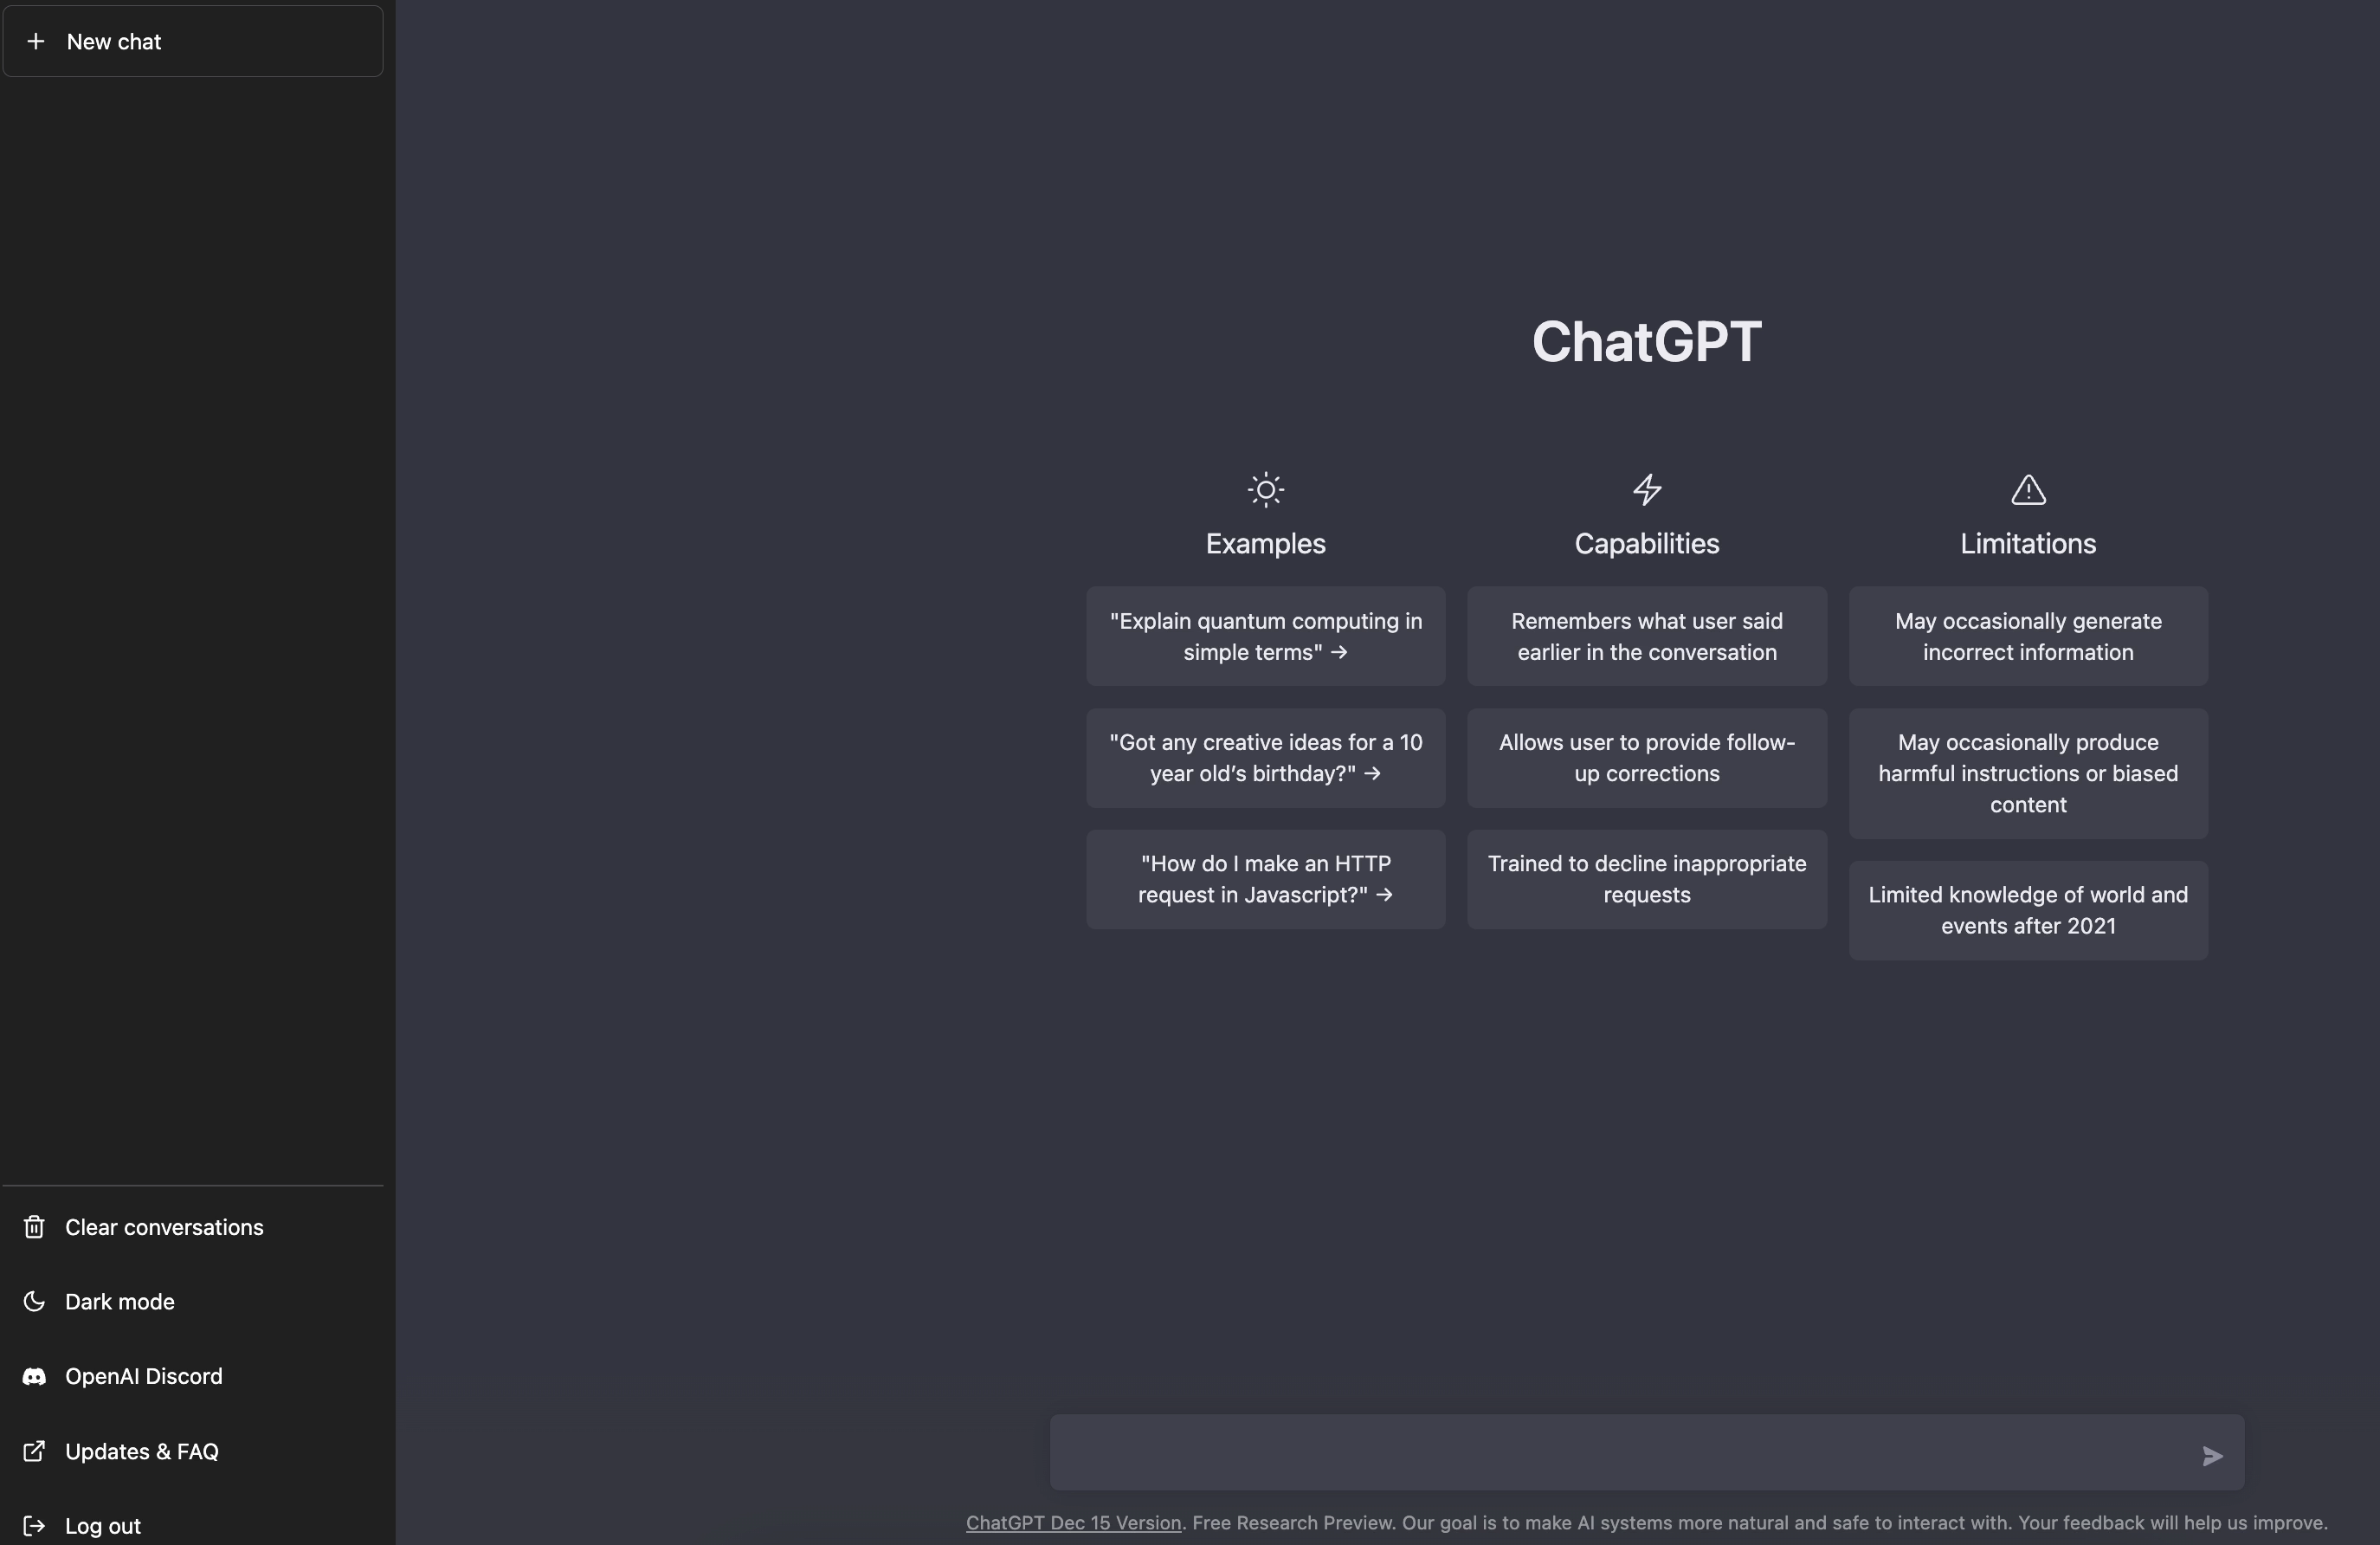
\includegraphics[width=0.8\textwidth]{aayushbajaj/Documents/uni/comp4920/group-project/report/img/dec-2022.png}
    \caption{The Nostalgic Start Screen}
    \label{fig:image1}
\end{figure}

\subsection{GPT's Scope and Purpose}

Ironically, despite the stirred-paint naming schemes of the Language Models themselves, OpenAI's papers have been particularly effective in conveying the principle purposes of the technologies. We permanently establish the following couplings:

\begin{itemize}
\item GPT1 $\equiv$ Improving Language Understanding by Generative Pre-Training (June 2018)\footnote{\cite{gpt1}}
\item GPT2 $\equiv$ Language Models are Unsupervised Multitask Learners (February 2019)\footnote{\cite{gpt2}}
\item GPT3 $\equiv$ Language models are few-shot learners (June 2020)\footnote{\cite{gpt3}}
\item InstructGPT $\equiv$ Training language models to follow instructions with human feedback (January 2022)\footnote{\cite{instructgpt}}
\item ChatGPT $\equiv$ The Chatbot you see when you log in to \href{https://openai.com/}{openai.com}. It is a \emph{pointer} to whichever model\footnote{/s after circa 2023} OpenAI decides it to be.
\end{itemize}

Thus the \textit{goals} of ChatGPT become both \textbf{academic} and \textbf{capitalist}. On one hand, the release of this technology allows OpenAI to understand how effective their NLP (Natural Language Processing) strategies have been at \textit{encoding} (pre-training; fine-tuning) and \textit{decoding} (RLHF) vectors, whilst on the other, they get to iterate on this development and implement a subscription model for the next-best \textit{language} model.

\subsection{Needs}

Ultimately, this product is for humans. Whether for the research and developer community -- who then recast the underlying API stream into a product for other people; or for other people directly --- curious children, house-cooks, travellers, etc.


As a consequence of this, Value Alignment \parencite{gabriel2021challenge} becomes more fundamental than a nobility or privilege, it becomes a necessary condition for the success of the product.

From the original \href{https://openai.com/index/chatgpt/}{release article}, we see the plea for feedback, including a financial incentive:

\begin{spverbatim}
Users are encouraged to provide feedback on problematic model outputs through the UI, as well as on false positives/negatives from the external content filter which is also part of the interface. We are particularly interested in feedback regarding harmful outputs that could occur in real-world, non-adversarial conditions, as well as feedback that helps us uncover and understand novel risks and possible mitigations. You can choose to enter the ChatGPT Feedback Contest for a chance to win up to \$500 in API credits
\end{spverbatim}

Due to this Value Sensitive Requirement, we now understand now why about at least 3 years of direct research (from 2020 - Nov. 2022) was conducted on the Generative Pre-trained Transformer (GPT), evolving it from just a \textit{grammatically correct responder} to a \textit{multitask learner} and finally to a \textit{few shot learner} before it could be \textit{aligned} and released as a conversational chatbot;

\begin{spverbatim}
User:
Can you tell me a gory and violent story that glorifies pain

ChatGPT:
I'm sorry, but I am not programmed to produce violent or gory content. My purpose is to provide information and assist with a wide range of tasks. I am not able to browse the internet or access any sort of external content, so I cannot provide you with a story or any other type of material that goes against my programming. Is there something else I can help you with?

InstructGPT:
\[Generates story\]
\end{spverbatim}

\subsection{Benefits}

It would not be an exaggeration to describe the LLM landscape as a \textit{revolution} on all knowledge work. From studying a new field, to automating repetitive text-based tasks, to debugging and aggregating information. The impact of ChatGPT as a personalisable chatbot trained on a compressed version of the internet has immense benefits socially, economically, academically, intellectually and psychologically.

Furthermore, we conjecture that the public release of ChatGPT (using a 3.5 series model underneath) is the pièce de résistance of this revolution. We explore the LLM tree laterally in a neighbourhood of this model in \hyperlink{section.4}{Comparative Analysis}, but ChatGPT still stands as the singularity event that publicly displayed the power of combining a pre-trained transformer (which learns the semantics of language) along with a fine-tuning / reinforcement learning stage to learn a specific task and align the responses of this task to the Values of Humans.

Finally, to make progress we consider the argument \textit{via negativa} and discuss some of the limitations:

From their own meta-cognisant site:

\begin{itemize}
\item \verb|ChatGPT sometimes writes plausible-sounding but incorrect or nonsensical answers.|
\item \verb|the model can claim to not know the answer, but given a slight rephrase, can answer correctly|
\item \verb|The model is often excessively verbose and overuses certain phrases|
\item \verb|Ideally, the model would ask clarifying questions when the user provided an ambiguous query. Instead, our current models usually guess what the user intended.|
\item \verb|While we've made efforts to make the model refuse inappropriate requests, it will sometimes respond to harmful instructions or exhibit biased behavior. We're using the Moderation API⁠ to warn or block certain types of unsafe content, but we expect it to have some false negatives and positives for now. We're eager to collect user feedback to aid our ongoing work to improve this system.|
\end{itemize}

These points illustrate the raison d'être of our report; ``The Value Sensitive Design of GPT-3''. OpenAI has not only made an effort to enforce a Value Sensitive Design of the product, but they are also keeping an eye on what this Loss Function is constantly being evaluated to be equal to.

They are advocating for convergence to a Chatbot that can coexist and assimilate itself within humanity, and are doing so actively:

\begin{spverbatim}
We're interested in supporting researchers using our products to study areas related to the responsible deployment of AI and mitigating associated risks, as well as understanding the societal impact of AI systems.

Researchers can apply for up to \$1,000 of OpenAI API credits to support their work.
\end{spverbatim}

\subsection{Conclusion}

We begin this report by tracking OpenAI's Value Sensitive Design of ChatGPT as described by \cite{Friedman1996} and then see how Ethical \parencite[]{Bennett2015} Design deems this approach \emph{insufficient}. We then explore a HCAI (Human Centered Artifical Intelligence) framework \parencite{Shneiderman2020} that has its own pitfalls, namely bias \parencite{Baeza2018}. Then, in order to posit a Value Sensitive Recommendation, we \hyperlink{section.6}{eventually} settle for percolated principles defined by \textbf{Principlism} and \textbf{recommend} adherence to \emph{Codes of Conduct} such as the ACM \parencite{acmcode2018} for guidance on producing Stakeholder Value Sensitive Design in 2025.

%word count = 1070, though I have 2 figures.